\part{Der Bruhat-Tits-Baum für $\GL_2$}

%===========
\section{$p$-adische Zahlen}\label{sec_padisch}

Es sei $p$ eine Primzahl. Eine Zahl $n\in\NN$ lässt sich eindeutig
schreiben als
\[
n = \SUM{k}{i=0} a_i p^i
\]
mit $a_i\in\{0,\ldots,p-1\}$ und $k\geq 0$.

\BEM\label{def_ubertrag}
Wir rechnen mit Übertrag: Für $n=\sum a_i p^i$ und
$m=\sum b_i p^i$ ist
\begin{gather*}
m+n = \sum c_i p^i, \\
mn = \sum d_i p^i
\end{gather*}
mit
$c_i = \tilde{c}_i - \rho_i p$,
$d_i = \tilde{d}_i - \sigma_i p$,
wobei 
\[
\tilde{c}_i=a_i+b_i+\rho_{i-1},\quad
\tilde{d}_i=(\sum_{l=0}^i a_l b_{i-l})+\sigma_{i-1}
\]
und
$\rho_i = \left\{\begin{matrix}
1, & \tilde{c}_i \geq p \\
0, & \tilde{c}_i < p
\end{matrix}\right.,$
$\sigma_i=\max\{s\in\NN:sp\leq \tilde{d}_i\}$
ist.

\DB Die Menge
\[
\ZZ_p = \left\{
\SUM{\infty}{i=0} a_i p^i : a_i \in \{0,\ldots,p-1\}
\right\}
\]
wird mit $+$ und $\cdot$ wie in Definition \ref{def_ubertrag}
zu einem kommutativen Ring mit $1$. Er heißt
\emph{Ring der ganzen $p$-adischen Zahlen}.\index{p-adische Zahlen!Ring}\index{$\ZZ_p$ ($p$-adische Zahlen)}

\bew Wir zeigen, dass $(\ZZ_p,+)$ eine Gruppe ist:
\begin{align*}
-(\sum a_i p^i) &= (p-a_0) + (p-a_1-1) p + (p-a_2-1) p^2 + \ldots \\
&= (p-a_0) + \SUM{\infty}{i=1} (p-a_i-1) p^i.
\end{align*}
Es gibt also zu jedem Element ein additiv Inverses.

Die übrigen Ringeigenschaften sind klar.
\qed

\PROP\ \begin{enumerate}
\item Die Inklusion $\NN\subset \ZZ_p$ induziert eine Einbettung
$\iota:\ZZ\hookrightarrow \ZZ_p$.
\item $\ZZ_p$ ist nullteilfrei.
\end{enumerate}
\bew \begin{enumerate}
\item Für $n\in\ZZ$, $n<0$, setze $\iota(n):=-\iota(-n)$.
\item Es seien $a=\sum a_i p^i, b=\sum b_i p^i \in \ZZ_p\backslash\{0\}$ und
\[
i_a := \min\{i:a_i \neq 0\},\quad
i_b := \min\{i:b_i \neq 0\}.
\]
Für $ab=\sum d_i p^i$ ist dann $\tilde{d}_{i_a+i_b}=a_{i_a}b_{i_b}$
nicht durch $p$ teilbar, da $p$ prim ist.
Folglich ist auch $d_{i_a+i_b}=\tilde{d}_{i_a+i_b}-\sigma_i p$
nicht durch $p$ teilbar und insbesondere $\neq 0$.
Also ist $ab\neq 0$.
\qed
\end{enumerate}

\BEM Es sei
\[
\mm_p = \left\{
a=\SUM{\infty}{i=0} a_i p^i \in \ZZ_p : a_0=0
\right\}.
\]
Dann gilt:
\begin{enumerate}
\item $\mm_p$ ist ein maximales Ideal.
\item $\ZZ_p/\mm_p \cong \ZZ/p\ZZ \cong \FF_p$.
\item $a\in \ZZ_p^\times$ genau dann, wenn $a\not\in\mm_p$.
\end{enumerate}
Insbesondere ist $\mm_p$ das einzige maximale Ideal in $\ZZ_p$,
d.h. $\ZZ_p$ ist ein lokaler Ring (vgl. Kapitel II.4 in 
Lang \cite{lang}).

\bew \begin{enumerate}
\item Offensichtlich ist $\mm_p$ ein Ideal. Die Maximalität
folgt aus Teil 2 oder 3.
\item Die Abbildung $a=\sum a_i p^i \mapsto \bar{a}_0\in \ZZ/p\ZZ$
ist ein surjektiver Ringhomomorphismus mit Kern $\mm_p$.
Der Homomorphiesatz liefert die Behauptung.
\item Es sei $a=\sum a_i p^i \in \ZZ_p\backslash \mm_p$, also
$a_0\neq 0$. Gesucht ist $b=\sum b_i p^i$ mit $ab=1$.
Definiere die $b_i$ induktiv: Da $p$ prim ist, kann man $b_0$ so 
wählen, dass $a_0 b_0 \equiv 1 \mod p$ gilt.
Hat man für $i\geq 1$ schon $b_0,\ldots,b_{i-1}$ gefunden, wähle
$b_i$ so, dass
\[
a_0 b_i + \SUM{i}{l=1} a_l b_{i-l} \equiv 0 \mod p
\]
gilt.
\qed
\end{enumerate}

\DB\
\begin{enumerate}
\item Der Quotientenkörper
\[
\QQ_p = \mathrm{Quot}(\ZZ_p)
\]
heißt \emph{Körper der $p$-adischen Zahlen}.\index{p-adische Zahlen!Körper}\index{$\QQ_p$ ($p$-adische Zahlen)}
\item Die Inklusion $\ZZ\hookrightarrow \ZZ_p$ induziert eine
Inklusion $\QQ\hookrightarrow \QQ_p$ (d.h. $\Char(\QQ_p)=0$).
\item Jedes $a\in \QQ_p^\times=\QQ_p\backslash\{0\}$ hat eine
eindeutige Darstellung
\[
a=\SUM{\infty}{i=i_a} a_i p^i
\]
mit $a_i\in\{0,\ldots,p-1\}$ und $i_a\in\ZZ$ minimal, so dass
$a_{i_a}\neq 0$.
\end{enumerate}
\textsc{Beweis von 3.:} Ist $a=\sum a_i p^i\in\ZZ_p\backslash\{0\}$,
so sei $i_a=\min\{i:a_i\neq 0\}$.
Dann ist $a=\SUM{\infty}{i=i_a} a_i p^i$ die gewünschte Darstellung.

Es ist $a=p^{i_a} u$ mit $u=\SUM{\infty}{i=0}a_{i+i_a} p^i\in\ZZ_p^\times$.
Nun sei $\frac{a}{b}\in\QQ_p$ mit $a,b\in\ZZ_p$, $b\neq 0$.
Schreibe $a=p^{i_a} u$ und $b=p^{i_b}v$ mit $i_a,i_b\in\NN$ und
$u,v\in\ZZ_p^\times$.
Es folgt
$\frac{a}{b}=p^{i_a-i_b} \ub{uv^{-1}}{\in\ZZ_p^\times}$,
wie gewünscht.
\qed

\DB\
\begin{enumerate}
\item Für $a=\SUM{\infty}{i=i_a}a_i p^i \in \QQ_p^\times$ sei
\begin{gather*}
\vv(a) := i_a,\\
|a| := p^{-i_a}.
\end{gather*}
\item Ist $a\in \ZZ$, so ist $\vv(a)=\max\{n:p^n|a\}$.
\item $a\in\ZZ_p\backslash\{0\}\ \lra\ \vv(a)\geq 0\ \lra\ |a|\leq 1$.
\item Setze $\vv(0):=\infty$, $|0|:=0$.
\item Für alle $a,b\in\QQ_p^\times$ gilt:
\begin{enumerate}
\item $\vv(ab)=\vv(a)+\vv(b)$ bzw. $|ab|=|a|\cdot |b|$.
\item $\vv(a+b)\geq\min\{\vv(a),\vv(b)\}$ bzw.
$|a+b|\leq\max\{|a|,|b|\}$.
\item Ist $\vv(a)\neq\vv(b)$, so ist $\vv(a+b)=\min\{\vv(a),\vv(b)\}$
bzw. $|a+b|=\max\{|a|,|b|\}$.
\item $\vv(a)=\vv(-a)$.
\end{enumerate}
\item $\vv:\QQ_p^\times \Ra \ZZ$ heißt \emph{$p$-adische Bewertung},
$|\cdot|:\QQ_p^\times \Ra \RR$ heißt \emph{$p$-adischer Betrag}.
\index{p-adische Bewertung}\index{p-adischer Betrag}\index{$\vv(a)$, $|a|$ ($p$-adische Bewertung)}
\end{enumerate}

\PROP\
\begin{enumerate}
\item $d(x,y):=|x-y|$ ist eine Metrik auf $\QQ_p$.
\item Jedes Dreieck in $\QQ_p$ ist gleichschenklig und die dritte
Seite ist höchstens so lang wie einer der gleichen Schenkel.
\end{enumerate}
\bew
\begin{enumerate}
\item Es gilt
\begin{gather*}
d(x,y)=0\ \lra\ x-y=0\ \lra\ x=y,\\
d(y,x)=|y-x|=|-(x-y)|=|-1|\cdot|x-y|=d(x,y)\\
\text{und}\\
d(x,z)=|x-z|=|(x-y)+(y-z)|\leq\max\{|x-y|,|y-z|\}\leq d(x,y)+d(x,z).
\end{gather*}
\item Folgt aus $|x-z|\leq \max\{|x-y|,|y-z|\}$.
\qed
\end{enumerate}

\PROP\ \begin{enumerate}
\item $\QQ_p$ ist vollständig.
\item $\QQ$ liegt dicht in $\QQ_p$.
\end{enumerate}
\bew \begin{enumerate}
\item Es sei $(a^{(n)})$ eine Cauchy-Folge in $\QQ_p$,
\[
a^{(n)} = \SUM{\infty}{i=i_a(n)} a_i^{(n)} p^i,
\]
mit $a_i^{(n)}\in\{0,\ldots,p-1\}$ und $i_a(n):=i_{a^{(n)}}$.
Es ist
\[
\vv(a^{(n)}) = i_a(n) \text{ und } |a^{(n)}|=p^{-i_a(n)}.
\]
Nun gilt
\[
|a^{(n)}-a^{(m)}| = p^{-\vv(n,m)}
\]
mit $\vv(n,m):=\min\{i:a_i^{(n)}\neq a_i^{(m)}\}$.
Folglich gibt es für jedes $i$ ein $n_0(i)$ mit $a^{(n)}_i=a^{(m)}_i$
für alle $n\geq n_0(i)$.
Da $a^{(n)}$ eine Cauchy-Folge ist, gibt es außerdem ein $i_0$
mit $a_i^{(n)}=0$ für $i<i_0$ und alle $n$.
Dann ist
\[
a = \SUM{\infty}{i=i_0} a_i^{(n_0(i))} \in \QQ_p
\]
der Grenzwert.
\item $\NN$ (und damit auch $\ZZ$) ist dicht in $\ZZ_p$, 
folglich ist auch $\QQ=\mathrm{Quot}(\ZZ)$ dicht in
$\QQ_p=\mathrm{Quot}(\ZZ_p)$.
\qed
\end{enumerate}

% ===============
\section{Der Baum für $\QQ_p$}\label{sec_baumQp}

\DEF Für $a\in \QQ_p$ und reelles $r>0$ sei
\[
\KU_r(a) := \{ b\in\QQ_p : |a-b|\leq r \}
\]
der \emph{Kreis}\index{Kreis!in $\QQ_p$}\index{$\KU_r(a)$ (Kreis in $\QQ_p$)}
um $a$ mit Radius $r$.

\BSP Kreise in $\QQ_p$.
\begin{enumerate}
\item $\KU_1(0)=\ZZ_p$.
\item $\KU_{1/p}(0)=\mm_p$.
\item $\KU_r(0)=\mm_p$ für alle $r$ mit $\frac{1}{p}\leq r < 1$.
\item $\KU_{1/p}(a)=\{ b\in\QQ_p:|b-a|<1 \}$, d.h. topologisch sind
offene und abgeschlossene Kreise in $\QQ_p$ nicht zu unterscheiden.
\end{enumerate}

\BEM Für Kreise $\KU_i=\KU_{r_i}(a_i)$, $i=1,2$, gilt:
\[
\KU_1\cap\KU_2=\emptyset\text{ oder }
\KU_1\subset \KU_2 \text{ oder }
\KU_2\subset \KU_1.
\]
Insbesondere ist $\KU_r(a)=\KU_r(b)$ für jedes $b\in\KU_r(a)$, d.h.
jeder Punkt in $\KU_r(a)$ ist Mittelpunkt.

\bew Es sei $a\in \KU_1\cap\KU_2$ und ohne Einschränkung
$r_1\leq r_2$. Dann gilt für $b\in \KU_1$:
\begin{align*}
d(b,a_2) &= |b-a_1+a_1-a+a-a_2| \\
&\leq \max\{\ub{|b-a_1|}{\leq r_1\leq r_2},
\ub{|a_1-a|}{\leq r_1\leq r_2},
\ub{|a-a_2|}{\leq r_2}\} \\
&\leq r_2.
\end{align*}
Also ist $b\in \KU_2$ und $\KU_1\subset \KU_2$.
\qed

Wir betrachten nun den Kreis $\KU=\KU_1(0)=\ZZ_p$.
Dieser Kreis enthält offensichtlich $\mm_p=\KU_{1/p}(0)$, also
die Elemente $a$ aus $\ZZ_p$ mit $a_0=0$.
\begin{center}
	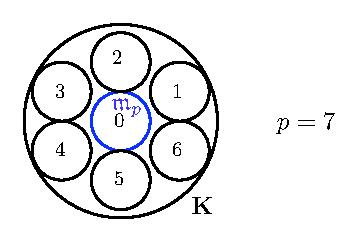
\includegraphics{grugraImages/kreisQp}
\end{center}
Für die übrigen Elemente von $\KU$ liegt $a_0\in\{1,\ldots,p-1\}$,
und $\KU$ enthält für jedes $a_0$ einen Kreis $\KU_{1/p}(i)$, dies
sind die Nebenklassen von $\mm_p$.
Die folgende Bemerkung verallgemeinert dies.

\BEM\ \label{bem_kreisQp}
\begin{enumerate}
\item Zu jedem Kreis $\KU=\KU_r(a)$ in $\QQ_p$ gibt es genau $p$
verschiedene maximale Kreise $\KU_1,\ldots,\KU_{p-1}$ mit
$\KU_i\subsetneq \KU$ für $i=1,\ldots,p-1$.
Es ist
\[
\KU_i = \KU_{r/p}(a+i p^{\lfloor\log_p(r)\rfloor}).
\]
\item Zu jedem Kreis $\KU=\KU_r(a)$ in $\QQ_p$ gibt es genau einen
minimalen Kreis $\KU'\supsetneq \KU$. Es ist
\[
\KU' = \KU_{rp}(a).
\]
\end{enumerate}

\DEF Es sei $T_p$ der Graph, der wie folgt definiert ist:
\begin{align*}
E(T_p) &= \{ \KU\subset\QQ_p : \KU \text{ ist Kreis} \}, \\
K(T_p) &= \{ (\KU,\KU') : \KU\subsetneq \KU' \text{ minimal oder }
\KU'\subsetneq \KU \text{ minimal} \},
\end{align*}
$\bar{(\KU,\KU')}=(\KU',\KU)$, $\ini(\KU,\KU')=\KU$ und
$\ter(\KU,\KU')=\KU'$.

Auf $T_p$ können wir eine kanonische Orientierung $K^+$ wählen,
indem wir aus jeder Kante $(\KU,\KU')$ den größeren der beiden Kreise
auswählen.\index{Orientierung}

\BEM $T_p$ ist ein Baum.

\bew $T_p$ ist zusammenhängend: Seien $\KU_i=\KU_{r_i}(a_i)$, $i=1,2$,
Kreise in $\QQ_p$. Ist $\KU_1\subset \KU_2$, so ist ohne Einschränkung
$a_1=a_2$ (denn jeder Punkt ist Mittelpunkt). Dann beschreibt
\[
\KU_1 \subset \KU_{r_1}p(a_1) \subset \ldots \subset
\KU_{r_1 p^k}(a_1)=\KU_2
\]
einen Weg in $T_p$.

$T_p$ enthält keine stachelfreien geschlossenen Wege: Wähle die
kanonische Orientierung $K^+$ auf $T_p$.
Es sei $w=(k_1,\ldots,k_n)$ ein stachelfreier Weg.
Beobachte, dass für $k_i\in K^-$ (d.h. $k_i=(\KU_i,\KU_{i+1})$
mit $\KU_i\subset \KU_{i+1}$) auch $k_{i+1},\ldots,k_n$ in $K^-$
liegen müssen (wegen Bemerkung \ref{bem_kreisQp}(2)).\\
Ist $w$ geschlossen, so gibt es ein $i$ mit $k_{i-1}\in\KU^+$ und
$k_i\in\KU^-$.
Folglich ist $\KU_{i-1}\subset \KU_i \supset \KU_{i+1}$, aber
$\KU_{i-1}\neq\KU_{i+1}$ (sonst gäbe es einen Stachel).
Also ist $\KU_{i-1}\cap \KU_{i+1}=\emptyset$. Wegen der obigen
Beobachtung ist $i$ eindeutig, also gilt
$\KU_0\subset \KU_{i-1}$ und $\KU_n\subset \KU_{i+1}$.
Und somit $\KU_0\neq \KU_n$, im Widerspruch dazu, dass $w$ geschlossen
sein soll. Somit kann $w$ nicht geschlossen sein.
\qed

\DEF Es sei $\GR$ ein Graph.
\begin{enumerate}
\item Ein \emph{Strahl}\index{Strahl} in $\GR$ ist ein Teilgraph,
der isomorph ist zu einer (in einer Richtung) unendlichen Kette.
\item Zwei Strahlen $R_1$ und $R_2$ heißen \emph{äquivalent}\index{Strahl!äquivalent},
wenn $R_1\cap R_2$ einen Strahl enthält.
\item Die Äquivalenzklassen von Strahlen heißen \emph{Enden}\index{Ende}.
\end{enumerate}
\begin{center}
	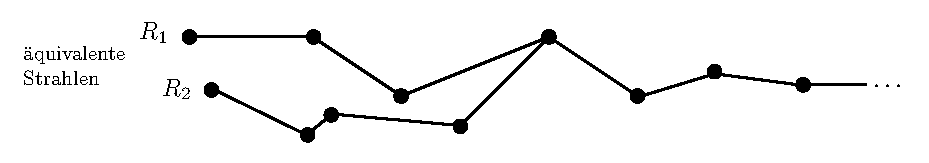
\includegraphics{grugraImages/R1R2}
\end{center}

\PROP Die Enden von $T_p$ entsprechen bijektiv den Punkten von
$\PP^1(\QQ_p)=\QQ_p\cup\{\infty\}$.\index{$\PP^1(\QQ_p)$ (projektiver Raum)}

\bew Suche eine Bijektion
\[
\phi:\{\text{Äquivalenzklassen von Strahlen in $T_p$}\}
\Ra \PP^1(\QQ_p).
\]
Es sei $R=(k_1,k_2,\ldots)$ ein Strahl in $T_p$.

Erster Fall: Alle $k_i\in K^+$. Setze $\phi(R):=\infty$.
Alle solchen Strahlen sind äquivalent.

Zweiter Fall: Fast alle $k_i\in K^-$ (d.h. alle ab einem $k_{i_0}$).
Es ist $\{a\}=\BCAP{}{i\geq i_0} \KU_i$.
Setze $\phi(R)=a$.

Man überzeugt sich leicht, dass $\phi$ wohldefiniert, surjektiv und
injektiv auf den Äquivalenzklassen von Strahlen ist.
\qed


\BEM
Die Achsen in $T_p$ entsprechen bijektiv den Punktpaaren
$\{x,y\}$ in $\PP^1(\QQ_p)$ (mit $x\neq y$).

\bew Es sei $A$ eine Achse in $T_p$. Zerlege $A$ in $R_1\cup R_2$
mit zwei Strahlen $R_1$ und $R_2$. Setze
\[
\psi(A) := \{\psi(R_1),\psi(R_2)\}
\]
für $\psi$ wie in Proposition \ref{prop_psi}.
Ist $A=\tilde{R}_1\cup\tilde{R}_2$ eine andere Zerlegung, so ist
$R_1\sim \tilde{R}_1$ und $R_2\sim\tilde{R}_2$ (oder umgekehrt),
also ist $\psi$ wohldefiniert.

$\psi$ ist injektiv: Es sei $A'=R_1'\cup R_2'$ mit
$\psi(A')=\psi(A)$, ohne Einschränkung sei $R_1\sim R_1'$ und
$R_2\sim R_2'$.
Wähle auf jedem Strahl die kanonische Orientierung (also die von
$K^+$ induzierte, von den Anfangspunkten wegweisende).
Dann enthalten $R_1$ und $R_2$ keine gleichorientierte Kante.\\
Angenommen, es ist $A\neq A'$. Dann gibt es ein $x\in E(A')$ mit
$x\not\in E(A)$. Ohne Einschränkung sei $x\in E(R_1')$.
Wähle $x'$ so, dass $R_1$ und $R_1'$ sich in $x'$ treffen.
Außerdem sei $y\in (E(R_2)\cap E(R_2'))\backslash E(R_1')$.
\begin{center}
	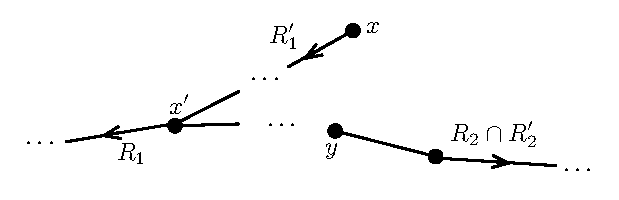
\includegraphics{grugraImages/strahlen}
\end{center}
Dann ist die Strecke $\bar{xy}$ in $A'$. Andererseits liegt $x'$
auf der Strecke $\bar{xy}$, aber $\bar{xx'}$ hat die Orientierung
von $R_1'$, wohingegen $\bar{xy}$ die Orientierung von $R_2'$ hat;
ein Widerspruch.

$\psi$ ist surjektiv: Zu je zwei Enden in $T_p$ gibt es eine Achse.
\qed

Im Folgenden werden wir Punkte aus $\PP^1(\QQ_p)$ mit
Enden von $T_p$ identifizieren, ohne die Bijektion 
$\psi$ explizit anzugeben.

\DB\ \label{bem_median}
\begin{enumerate}
\item Es sei $T$ ein Baum, $e_1,e_2,e_3$ seien drei verschiedene
Enden von $T$ und $A_{ij}$ die durch $e_i,e_j$ bestimmte Achse.
Dann gibt es $x=\med(e_1,e_2,e_3)$ mit
$\{x\}=E(A_{12})\cap E(A_{13})\cap E(A_{23})$.
Wir nennen $\med(e_1,e_2,e_3)$ den \emph{Median}\index{Median}\index{$\med(a,b,c)$ (Median)}
der Enden $e_1$, $e_2$ und $e_3$.
\item Es seien $a,b,c\in\PP^1(\QQ_p)$ und ohne Einschränkung
$|a-b|\leq\min\{|a-c|,|b-c|\}$ und $|a|\leq |b|$.
Dann ist $\med(a,b,c)=\KU_{|a-b|}(a)$.
\end{enumerate}

\bew\ \begin{enumerate}
\item Es seien zunächst $e_1,e_2,e_3\in E(T)$ und
$A_{ij}=\bar{e_i e_j}$ der stachelfreie Weg von $e_i$ nach $e_j$.
Weiter sei $w_i=K(A_{ij})\cap K(A_{ik})$ ein Weg mit Anfangspunkt
$x_i$ und es sei $y_i=\ter(w_i)$.
Dann liegt $\bar{y_i y_j}$ in $A_{ij}$, und für jede Kante $k$ von
$\bar{y_i y_j}$ gilt: $k\not\in K(A_{ik})\cup K(A_{jk})$.
Also ist $\bar{y_1 y_2}\cdot\bar{y_2 y_3}\cdot\bar{y_3 y_1}$
ein stachelfreier
geschlossener Weg. Da $T$ aber ein Baum ist, folgt $y_1=y_2=y_3$.\\
Sind nun $e_1,e_2,e_3$ Enden von $T$, so sei
$y_i\in (E(A_{ij})\cap E(A_{ik}))\backslash E(A_{jk})$. Dann liegt
$x=\med(y_1,y_2,y_3)$ im Schnitt der Wege $\bar{y_1 y_2}$,
$\bar{y_2 y_3}$ und $\bar{y_1 y_3}$, d.h.
\[
x \in E(A_{12})\cap E(A_{13}) \cap E(A_{23}).
\]
\item
Zuerst der Fall $c=\infty$ (nach Voraussetzung kann von $a$, $b$ und
$c$ nur
$c$ diesen Wert annehmen):
\begin{center}
	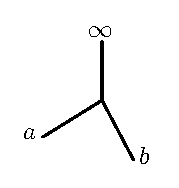
\includegraphics{grugraImages/enden1}
\end{center}
Es ist
\begin{align*}
E(A_{a,\infty}) &= \{\KU_r(a) : r=p^k, k\in\ZZ \}, \\
E(A_{b,\infty}) &= \{\KU_r(b) : r=p^k, k\in\ZZ \}
\end{align*}
und folglich
\[
\med(a,b,c)=\KU_{|a-b|}(a)=\KU_{|a-b|}(b).
\]
Es ist $E(A_{a,b})=\{\KU_r(a):r\leq |a-b|\}\cup
\{\KU_r(b):r\leq|a-b|\}$.

Nun zum Fall $c\neq\infty$:
\begin{center}
	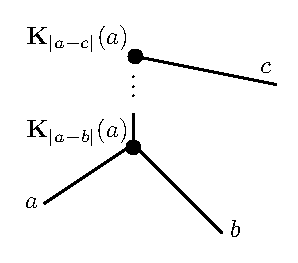
\includegraphics{grugraImages/enden2}
\end{center}
Nach Voraussetzung ist $|a-c|\geq |a-b|$ und $|b-c|\geq |a-b|$.
\qed
\end{enumerate}


% ==================
\section{Die Aktion von $\PGL_2(\QQ_p)$ auf $T_p$}\label{sec_PGL}

\BEM Es sei $\KK$ ein beliebiger Körper.
\begin{enumerate}
\item Die Gruppe $\GL_2(\KK)$ operiert auf
\[
\PP^1(\KK) := \KK \cup \{\infty\}
\]
durch die Möbiustransformation\index{Möbiustranformation}
\[
\begin{pmatrix}
a & b \\
c & d
\end{pmatrix}\cdot z
:=
\left\{
\begin{matrix}
\frac{az+b}{cz+d}, & z\in\KK, cz+d\neq 0 \\
\infty, & z\in\KK, cz+d = 0 \\
\frac{a}{c}, & z=\infty
\end{matrix}
\right..
\]
Der Fall \glqq$\frac{0}{0}$\grqq\ kann wegen $ad-cb\neq 0$ nicht
vorkommen.
\item Der Ineffektivitätskern der Aktion ist
\[
\{ \lambda I_2 : \lambda\in\KK^\times \}.
\]
\end{enumerate}
\bew \begin{enumerate}
\item Für $A,B\in\GL_2(\KK)$ erhält man $A(B\cdot z)=(AB)\cdot z$
durch direktes Nachrechnen.
\item
\glqq$\subseteq$\grqq:
Es sei $\frac{az+b}{cz+d} = z$ für alle $z\in\PP^1(\KK)$.
Dann:
\begin{align*}
&z=0\ \ra\ \frac{b}{d}=0\ \ra\ b=0, \\
&z=\infty\ \ra\ \frac{a}{c}=\infty\ \ra\ c=0, \\
&z=1\ \ra\ \frac{a}{d}=1\ \ra\ a=d.
\end{align*}
\glqq$\supseteq$\grqq: Klar.
\qed
\end{enumerate}

\FOLG Die \emph{projektive lineare Gruppe}\index{projektive Gruppe}
\[
\PGL_2(\KK) := \GL_2(\KK)\left/\{ \lambda I_2 : \lambda\in\KK^\times\}\right.
\]
operiert effektiv auf $\PP^1(\KK)$.

\PROP Für $a,b,c\in\PP^1(\QQ_p)$ paarweise verschieden und
$\gamma\in\PGL_2(\QQ_p)$ sei
\[
\gamma(\med(a,b,c)) := \med(\gamma(a),\gamma(b),\gamma(c)).
\]
Dadurch wird eine Aktion von $\PGL_2(\QQ_p)$ auf $T_p$ definiert.

\bew Es seien $a,b,c$ wie in Bemerkung
\ref{bem_median}.
\begin{itemize}
\item Zuerst zeigen wir die Wohldefiniertheit:
Ist $\med(a',b',c')=\med(a,b,c,)$, so ist
\[
\med(\gamma(a'),\gamma(b'),\gamma(c'))
=\med(\gamma(a),\gamma(b),\gamma(c))
\qquad (*)
\]
für alle $\gamma\in\PGL_2(\QQ_p)$ zu zeigen.
Es reicht, dies für Erzeuger von $\PGL_2(\QQ_p)$ zu zeigen.
Dazu schreiben wir
\[
\gamma = \begin{pmatrix} a_1 & a_2 \\ a_3 & a_4 \end{pmatrix}
=
\left\{\begin{matrix}
\begin{pmatrix} 1 & 0 \\ \frac{a_3}{a_1} & 1 \end{pmatrix}
\begin{pmatrix} a_1 & 0 \\ 0 & \frac{\det(\gamma)}{a_1} \end{pmatrix}
\begin{pmatrix} 1 & a_2 \\ 0 & 1 \end{pmatrix}, & a_1\neq 0 \\ \\
\begin{pmatrix} 0 & 1 \\ 1 & 0 \end{pmatrix}
\begin{pmatrix} a_3 & 0 \\ 0 & a_2 \end{pmatrix}
\begin{pmatrix} 1 & a_4 \\ 0 & 1 \end{pmatrix}, & a_1=0
\end{matrix}\right..
\]
Außerdem ist
\[
\begin{pmatrix} 1 & 0 \\ y & 1 \end{pmatrix}
=
\begin{pmatrix} 0 & 1 \\ 1 & 0 \end{pmatrix}
\begin{pmatrix} 1 & y \\ 0 & 1 \end{pmatrix}
\begin{pmatrix} 0 & 1 \\ 0 & 1 \end{pmatrix}.
\]
Wir müssen $(*)$ also nur für
\begin{align*}
&z\mapsto \lambda z,\quad \lambda \in \QQ_p^\times, \\
&z\mapsto z+z_0,\quad z_0 \in \QQ_p, \\
&z\mapsto\frac{1}{z}
\end{align*}
zeigen.
Dazu seien $a',b',c'$ gegeben mit $\med(a,b,c)=\med(a',b',c')$
und $|a'-b'|\leq\min\{|a'-c'|,|b'-c'|\}$.
Dann ist
$\med(a,b,c)=\KU_{|a-b|}(a)=\KU_{|a'-b'|}(a')=\med(a',b',c')$ und
folglich $|a-b|=|a'-b'|$ und $|a'-a|\leq|a-b|$.
Wir betrachten nun die drei Fälle einzeln:

Der Fall $z\mapsto \lambda z$: Es ist
\[
\med(\lambda a,\lambda b,\lambda c)
=\KU_{|\lambda|\cdot|a-b|}(\lambda a)
=\KU_{|\lambda|\cdot|a'-b'|}(\lambda a')
=\med(\lambda a',\lambda b',\lambda c'),
\]
wobei die Gleichheit in der Mitte sich aus
$|\lambda a'-\lambda a|=|\lambda|\cdot|a'-a|\leq|\lambda|\cdot|a-b|$
ergibt.

Der Fall $z\mapsto z+z_0$: Es ist
\begin{gather*}
\med(a+z_0,b+z_0,c+z_0) = \KU_{|a-b|}(a+z_0), \\
\med(a'+z_0,b'+z_0,c'+z_0) = \KU_{|a'-b'|}(a'+z_0).
\end{gather*}

Der Fall $z\mapsto\frac{1}{z}$: Wir schreiben $r:=|a-b|$.\\
Zunächst sei $|a|\leq r$. Dann ist auch $|b|\leq r$, $|c|\geq r$ und
$\KU_r(a)=\KU_r(0)$. Gesucht ist
\[
\min\Bigl\{
\Bigl| \ub{\frac{1}{a}-\frac{1}{b}}{=\frac{r}{|a|\cdot|b|}} \Bigr|,
\Bigl| \ub{\frac{1}{a}-\frac{1}{c}}{=\frac{|a-c|}{|a|\cdot|c|}} \Bigr|,
\Bigl| \ub{\frac{1}{b}-\frac{1}{c}}{=\frac{|b-c|}{|b|\cdot|c|}} \Bigr|
\Bigr\}.
\]
Mit Hilfe von Proposition \ref{prop_schenkel}(2) und der folgenden
(nicht maßstabsgetreuen) Skizze kann man dies herleiten.
\begin{center}
	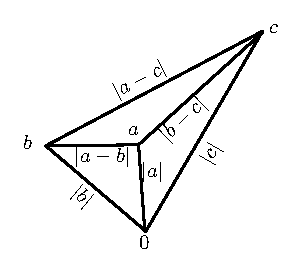
\includegraphics{grugraImages/abc}
\end{center}
Es muss $|a-c|=|c|=|b-c|$ gelten und außerdem $|b|=r\geq |a|$.
Dann ist
\[
\frac{r}{|a|\cdot |b|}\geq \frac{1}{|a|}=\frac{|a-c|}{|a|\cdot|c|}
=\frac{|b-c|}{|a|\cdot|c|}\geq\frac{|b-c|}{|b|\cdot|c|}.
\]
Also ist das gesuchte Minimum
$|\frac{1}{b}-\frac{1}{c}|=\frac{1}{|b|}$. Es folgt
$\med(\frac{1}{a},\frac{1}{b},\frac{1}{c})=\KU_{1/r}(\frac{1}{b})
=\KU_{1/r}(0)$. Genauso kann man für $a'$, $b'$ und $c'$ argumentieren
und man erhält
$\med(\frac{1}{a'},\frac{1}{b'},\frac{1}{c'})=\KU_{1/r}(\frac{1}{b'})
=\KU_{1/r}(0)$.\\
Nun sei $|a|>r$. Dann ist $|a|=|b|$ und
$|\frac{1}{a}-\frac{1}{b}|=\frac{r}{|a|^2}$. Ist $|c|<|a-c|=|a|$,
so gilt
\[
\Bigl|\frac{1}{a}-\frac{1}{c}\Bigr|=\frac{|a-c|}{|a|\cdot|c|}
=\frac{1}{|c|}
\]
und somit $\frac{1}{|c|}>\frac{r}{|a|^2}$. Andernfalls ist
$\frac{|a-c|}{|a|\cdot|c|}\geq\frac{r}{|a|^2}$, da entweder
$|c|=|a|$ oder $|c|=|a-c|$. Es folgt
$\med(\frac{1}{a},\frac{1}{b},\frac{1}{c})
=\KU_{r/|a|^2}(\frac{1}{a})$. Es ist
\[
\KU_{|a'-b'|}(a')=\med(a',b',c')=\med(a,b,c)=\KU_r(a),
\]
also $a'\in\KU_r(a)$ und $|a-a'|\leq r < |a|$. Es folgt $|a|=|a'|$.
Es ist $\med(\frac{1}{a'},\frac{1}{b'},\frac{1}{c'})
=\KU_{r/|a'|^2}(\frac{1}{a'})$, und da
\[
\frac{|a-a'|}{|a|\cdot|a'|}=\Bigl|\frac{1}{a}-\frac{1}{a'}\Bigr|
=\frac{r}{|a|^2},
\]
folgt wie vorhin $\KU_{r/|a'|^2}(\frac{1}{a'})=\KU_{r/|a|^2}(\frac{1}{a})$.
Eine Skizze für die Operation von $z\mapsto\frac{1}{z}$:
\begin{center}
	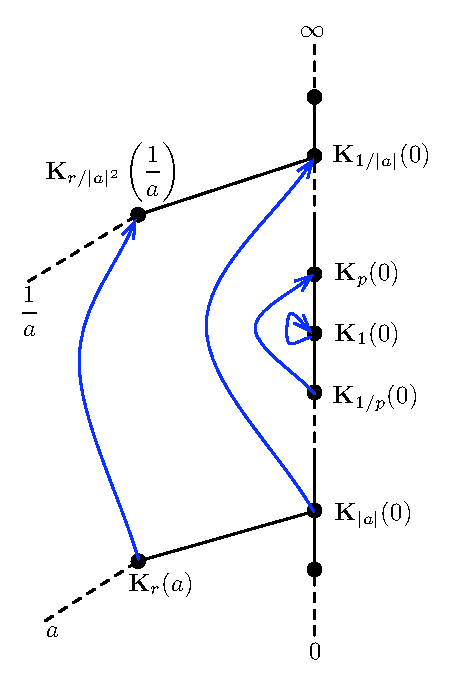
\includegraphics{grugraImages/pglAktion}
\end{center}
\item Nun zeigen wir, dass $\PGL_2(\QQ_p)$ auf den Kanten von $T_p$
operiert, d.h. dass benachbarte Ecken auf benachbarte Ecken abgebildet
werden. Auch hier reicht es, die drei Erzeugertypen zu betrachten.

Für $z\mapsto \lambda z$: Es wird $\KU_r(a)$ auf
$\KU_{|\lambda|r}(\lambda a)$ abgebildet und $\KU_{pr}(a)$ auf
$\KU_{|\lambda|pr}(\lambda a)$.

Für $z\mapsto z+z_0$: Es wird $\KU_r(a)$ auf $\KU_r(a+z_0)$
abgebildet und $\KU_{pr}(a)$ auf $\KU_{pr}(a+z_0)$.

Für $z\mapsto\frac{1}{z}$: Es wird $\KU_r(0)$ auf
$\KU_{1/r}(0)$ abgebildet und $\KU_{pr}(0)$ auf
$\KU_{1/(pr)}(0)$. Hierbei wird die Orientierung vertauscht:
\begin{center}
	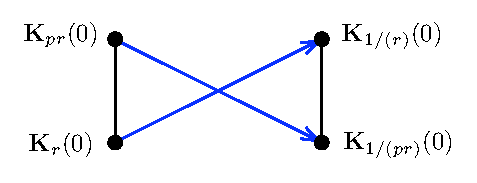
\includegraphics{grugraImages/vertauscht}
\end{center}
Ist $0\not\in \KU_{pr}(a)$, so geht $\KU_{r}(a)$ auf
$\KU_{r^2/|a|}(\frac{1}{a})$ und $\KU_{pr}(a)$ auf
$\KU_{pr/|a|^2}(\frac{1}{a})$.
\qed
\end{itemize}

\BEM $\PGL_2(\QQ_p)$ operiert transitiv auf den Ecken $E(T_p)$
und auf den Kanten $K(T_p)$, aber nicht inversionsfrei.

\bew $\PGL_2(\QQ_p)$ operiert transitiv auf den Tripeln verschiedener
Punkte $(a,b,c)\in\PP^1(\QQ_p)$, also insbesondere auf $E(T_p)$.

$z\mapsto pz$ bildet $(\KU_{1/p}(0),\KU_1(0))$ auf
$(\KU_1(0),\KU_p(0))$ ab.\\
$z\mapsto (1-n)z+n$ (mit $n=1,\ldots,p-1$) bildet
$\KU_1(0)=\med(0,1,\infty)$ auf $\med(n,1,\infty)=\KU_1(0)$ ab,
und $\KU_{1/p}(0)=\med(0,p,\infty)$ auf $\med(n,n+(1-n)p,\infty)
=\KU_{1/p}(0)$.

$z\mapsto \frac{p}{z}$ vertauscht $\KU_1(0)$ mit $\KU_{1/p}(0)$,
daher ist die Aktion nicht inversionsfrei.
\qed

\FOLG Es sei $T_p^*$ die baryzentrische Unterteilung von $T_p$.\index{$T_p^*$ (Unterteilung von $T_p$)}\index{Unterteilung}\index{baryzentrische Unterteilung}
Dann operiert $\PGL_2(\QQ_p)$ inversionsfrei auf $T_p^*$ mit dem
Quotientengraphen
\begin{center}
	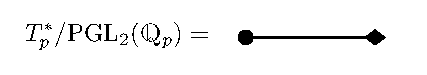
\includegraphics{grugraImages/pglQuotient}
\end{center}
Also ist $\PGL_2(\QQ_p) = G_1 *_{G_0} G_2$, wobei $G_1$ die Fixgruppe
von $\KU_1(0)$ ist und $G_0$ der Schnitt von $G_1$ mit
der Fixgruppe
von $\KU_{1/p}(0)$. Die Gruppe $G_2$ ist die Fixgruppe der Ecke
$\blacklozenge$.

$T_p^*$ ist enthalten im Bruhat-Tits-Baum für $\QQ_p(\sqrt{p})$.

Einen weiteren Zugang zur inversionsfreien Aktion erhält man
durch die Aktion einer Untergruppe von $\PGL_2(\QQ_p)$.

\BEM Die \emph{spezielle projektive Gruppe}\index{projektive Gruppe!spezielle}
\[
\PSL_2(\QQ_p) := \SL_2(\QQ_p)/\{\pm I_2\}
\]
hat Index $4$ in $\PGL_2(\QQ_p)$.

\bew Für $A\in\GL_2(\QQ_p)$ und $\lambda\in\QQ_p^\times$ ist
$\det(\lambda A)=\lambda^2\det(A)$, d.h. ein Element aus
$\PGL_2(\QQ_p)$ ist äquivalent zu einem Element aus
$\PSL_2(\QQ_p)$, wenn es als Repräsentanten eine Matrix hat,
deren Determinante ein Quadrat in $\QQ_p^\times$ ist.\\
Was ist nun $|\QQ_p^\times/(\QQ_p^\times)^2|$?
Schreibe $a\in \QQ_p^\times$ als $a=up^n$ mit $n\in\ZZ$,
$u\in\ZZ_p^\times$. Da $\sqrt{p}\not\in\QQ_p$, ist $p$ kein Quadrat
in $\QQ_p$.
Es ist $a\in(\QQ_p^\times)^2$ genau dann,
wenn $n\in 2\ZZ$ und $u\in(\ZZ_p^\times)^2$. Es sei
$\bar{u}\in\FF_p^\times$ das Bild von $u$ in $\FF_p$.
Es ist $|\FF_p^\times/(\FF_p^\times)^2|=2$. Mit dem Lemma von Hensel
(van der Waerden \cite{vdW}, § 144)
folgt, dass genau dann $u\in(\ZZ_p^\times)^2$ gilt, wenn
$\bar{u}\in(\FF_p^\times)^2$.
\qed

\FOLG Es sei $u\in\ZZ_p^\times\backslash(\ZZ_p^\times)^2$. Dann sind
\[
\begin{pmatrix}
1 & 0 \\
0 & 1
\end{pmatrix},
\begin{pmatrix}
u & 0 \\
0 & 1
\end{pmatrix},
\begin{pmatrix}
p & 0 \\
0 & 1
\end{pmatrix},
\begin{pmatrix}
pu & 0 \\
0 & 1
\end{pmatrix}
\]
Vertreter der Nebenklassen von $\PSL_2(\QQ_p)$ in $\PGL_2(\QQ_p)$.

\PROP Es gilt
\[
G_1 = \PGL_2(\QQ_p)_{\KU_1(0)} = \PSL_2(\ZZ_p).
\]
\bew
\glqq$\supseteq$\grqq:
Es sei $A=\begin{pmatrix}
a & b \\
c & d
\end{pmatrix}
\in\GL_2(\ZZ_p)$, d.h. $|a|\leq 1$, $|b|\leq 1$, $|c|\leq 1$,
$|d|\leq 1$ und $|ad-bc|=1$.
Zu zeigen ist
$A\cdot\KU_1(0)=\med(\frac{b}{d},\frac{a}{c},\frac{a+b}{c+d})
=\KU_1(0)$.

Zunächst nehmen wir an, dass es einen Matrixeintrag $<1$ gibt.
Ohne Einschränkung sei $|c|<1$ (dies lässt sich durch Anwenden einer
Permutation $S=\begin{pmatrix}
0 & 1 \\
1 & 0
\end{pmatrix}$
erreichen, und da $S\in\PSL_2(\ZZ_p)$ liegt und $\KU_1(0)$ 
stabilisiert, genügt es $A$ oder $SA$ oder $AS$ oder $SAS$ zu
betrachten).
Es gilt dann $|a|=|d|=1$, $|\frac{a}{c}|>1$,
$|\frac{b}{d}|=|b|\leq 1$, $|\frac{a+b}{c+d}|=|a+b|\leq 1$ und
$|\frac{b}{d}-\frac{a+b}{c+d}|=|bc+bd-ad-bd|=1$.
Also ist $\med(\frac{b}{d},\frac{a}{c},\frac{a+b}{c+d})=\KU_1(0)$.

Nun sei $|a|=|b|=|c|=|d|=1$.
Dann gilt $|\frac{b}{d}|=1=|\frac{a}{c}|$,
$|\frac{b}{d}-\frac{a}{c}|=\frac{|bc-ad|}{|d|\cdot|c|}=1$,
$|\frac{a+b}{c+d}-\frac{a}{c}|\geq 1$ und
$|\frac{a+b}{c+d}-\frac{b}{a}|\geq 1$. Also ist
$\med(\frac{b}{d},\frac{a}{c},\frac{a+b}{c+d})=\KU_1(0)$.

\glqq$\subseteq$\grqq:
Es sei $A=\begin{pmatrix}
a & b \\
c & d
\end{pmatrix}$ ein Repräsentant von $\gamma\in G_1$.
Ohne Einschränkung sei $|\det(A)|=1$ oder $|\det(A)|=\frac{1}{p}$.
Nach Voraussetzung ist
$\med(\frac{b}{d},\frac{a+b}{c+d},\frac{a}{c})=\KU_1(0)$.
Ohne Einschränkung dürfen wir
$\med(\frac{b}{d},\frac{a+b}{c+d},\frac{a}{c})
=\KU_{|\frac{b}{d}-\frac{a+b}{c+d}|}(\frac{b}{d})
=\KU_{|\gamma(0)-\gamma(1)|}(\gamma(0))$ annehmen
(denn wäre dies nicht so, könnte man es durch Anwenden der Untergruppe
\[
\Bigl\{z\mapsto z,\ z\mapsto\frac{1}{z},\
 z\mapsto 1-z,\ z\mapsto 1-\frac{1}{z},\
 z\mapsto \frac{z}{z-1},\ z\mapsto\frac{1}{1-z}
 \Bigr\}
 < \PGL_2(\QQ_p)
\]
erreichen, die $\{0,1,\infty\}$ auf sich abbildet).
Es gilt also $|\frac{b}{d}|\leq 1$, $|\frac{a+b}{c+d}|\leq 1$,
$|\frac{b}{d}-\frac{a+b}{c+d}|=1$, $|\frac{b}{d}-\frac{a}{c}|\geq 1$
und $|\frac{a}{c}-\frac{a+b}{c+d}|\geq 1$.
Daraus folgt
$|b|\leq |d|$, $|a+b|\leq|c+d|$, $|d|\cdot|c+d|=|ad-bc|$,
$|d|\cdot|c|\leq|ad-bc|$ und $|c|\cdot|c+d|\leq|ad-bc|$.\\
Nun muss $|d|=|c+d|$ sein, denn für $|d|<|c+d|$ gilt $|c|=|c+d|$
und
\[
|ad-bc|=|d|\cdot|c+d|<|c+d|^2=|c|\cdot|c+d|\leq|ad-bc|,
\]
und im Falle $|d|>|c+d|$ gilt $|c|=|d|$ und
\[
|ad-bc|=|d|\cdot|c+d|<|c|\cdot|d|\leq|ad-bc|,
\]
in beiden Fällen ein Widerspruch.
Aus $|d|=|c+d|$ folgt $|d|^2=|ad-bc|$ (da $\frac{1}{p}$ kein Quadrat 
ist). Es folgt
\[
|d|=1,\ |b|\leq 1,\ |c|\leq 1,\ |a|\leq 1,
\]
also $A\in\GL_2(\ZZ_p)$.
\qed

\FOLG\ \begin{enumerate}
\item Die Fixgruppe $G_0$ der Kante $(\KU_1(0),\KU_{1/p}(0))$
wird durch Matrizen
\[
\Bigl\{
\begin{pmatrix}
a & b \\
c & d
\end{pmatrix}\in\PGL_2(\ZZ_p) : |b|<1
\Bigr\}
\]
repräsentiert.
\item Der Index ist $[G_1:G_0]=p+1$.
\end{enumerate}
\bew \begin{enumerate}
\item Es ist
\[
\PGL_2(\QQ_p)_{\KU_1(0)}
=\gamma\cdot\PGL_2(\QQ_p)_{\KU_{1/p}(0)}\cdot\gamma^{-1}
\]
mit $\gamma=\begin{pmatrix}
p & 0 \\
0 & 1
\end{pmatrix}$.
Dies sind die Matrizen
\[
\Bigl\{
\begin{pmatrix}
p & 0 \\
0 & 1
\end{pmatrix}
\begin{pmatrix}
a & b \\
c & d
\end{pmatrix}
\begin{pmatrix}
\frac{1}{p} & 0 \\
0 & 1
\end{pmatrix}
=\begin{pmatrix}
a & pb \\
\frac{c}{p} & d
\end{pmatrix}:
\begin{pmatrix}
a & b \\
c & d
\end{pmatrix}\in\GL_2(\ZZ_p)
\Bigr\}.
\]
Folglich ist
\[
G_0 = \PGL_2(\ZZ_p) \cap \gamma\cdot\PGL_2(\ZZ_p)\cdot\gamma^{-1}
=
\Bigl\{
\begin{pmatrix}
a & b \\
c & d
\end{pmatrix}\in\PGL_2(\ZZ_p):|b|<1
\Bigr\}.
\]
\item Es sei $\phi:\PGL_2(\ZZ_p)\Ra\PGL_2(\FF_p)$ die von
$\phi:\ZZ_p\Ra\FF_p$ induzierte Abbildung. Damit ist
\[
G_0=\phi^{-1}\Bigl(
\ub{\Bigl\{
\begin{pmatrix}
* & 0 \\
* & *
\end{pmatrix}
\in\PGL_2(\FF_p)
\Bigr\}}{=:\PGL_2^0(\FF_p)}
\Bigr).
\]
Es ist
\begin{align*}
[G_1:G_0] &= [\PGL_2(\FF_p):\PGL_2^0(\FF_p)] \\
&= [\GL_2(\FF_p):\GL_2^0(\FF_p)] \\
&=\frac{(p^2-1)(p^2-p)}{(p-1)(p^2-p)} \\
&=p+1,
\end{align*}
wie behauptet.
\qed
\end{enumerate}

\PROP Es ist
\[
G_2 = \Bigl\lag \PGL_2^0(\ZZ_p),
\begin{pmatrix}
0 & p \\
1 & 0
\end{pmatrix}
\Bigr\rag
\leq\PGL_2(\QQ_p)
\]
und $[G_2:\PGL_2^0(\ZZ_p)]=2$.

\bew Es ist $\begin{pmatrix}
0 & p \\
1 & 0
\end{pmatrix}$ in der Fixgruppe von $\blacklozenge$, also
$\Bigl\lag \PGL_2^0(\ZZ_p),
\begin{pmatrix}
0 & p \\
1 & 0
\end{pmatrix}
\Bigr\rag\leq G_2$. Ist umgekehrt $\gamma\in
G_2\backslash\PGL_2^0(\ZZ_p)$, so ist
$\gamma\cdot
\begin{pmatrix}
0 & p \\
1 & 0
\end{pmatrix}
\in\PGL_2^0(\ZZ_p)$.
\qed

Zusammengefasst erhalten wir den folgenden Satz:

\SATZ Es ist
\[
\PGL_2(\QQ_p) =
\PGL_2(\ZZ_p) *_{\PGL_2^0(\ZZ_p)} \Bigl\lag \PGL_2^0(\ZZ_p),
\begin{pmatrix}
0 & p \\
1 & 0
\end{pmatrix}
\Bigr\rag.
\]


Nun betrachten wir die Aktion von $\SL_2(\QQ_p)$ auf $T_p$.

\FOLG Es ist
\[
\SL_2(\QQ_p) \cong \SL_2(\ZZ_p) *_{\SL_2^0(\ZZ_p)} \SL_2(\ZZ_p).
\]
(Dabei ist der zweite Faktor durch Konjugation
isomorph zu $\SL_2(\ZZ_p)$.)

\bew Der Stabilisator von $\KU_1(0)$ in $\PSL_2(\QQ_p)$
ist 
\[
\PGL_2(\ZZ_p)\cap\PSL_2(\QQ_p)=\PSL_2(\ZZ_p).
\]

Wir zeigen nun, dass das Segment
\begin{center}
	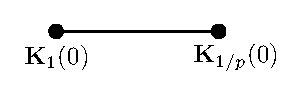
\includegraphics{grugraImages/Kkante}
\end{center}
ein Fundamentalbereich für die Aktion von $\SL_2(\QQ_p)$ auf $T_p$
ist. Wir schreiben abkürzend $x=\KU_1(0)$ und $y=\KU_{1/p}(0)$.
\begin{itemize}
\item $x$ und $y$ liegen in verschiedenen Bahnen von $\SL_2(\QQ_p)$.
Es ist nämlich $y=Bx$ mit
$B=\begin{pmatrix} p&0\\ 0&1 \end{pmatrix}\not\in\SL_2(\QQ_p)$.
Gäbe es ein $A\in\SL_2(\QQ_p)$ mit $Ax=y$, so wäre
$A^{-1} B x = x$, also $A^{-1}B$ im Stabilisator $\GL_2(\ZZ_p)$
von $x$. Dies ist ein Widerspruch, da
$\det(A^{-1}B)=p\not\in\ZZ_p^\times$.
\item Schreibe $\KU_i:=\KU_{1/p}(i)$ für $i=0,\ldots,p-1$.
\begin{center}
	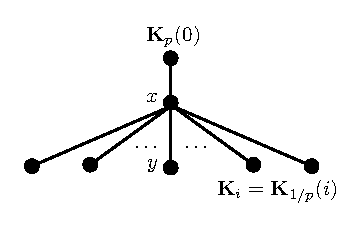
\includegraphics{grugraImages/Ki}
\end{center}
Die Matrix
$A_i=\begin{pmatrix} 1&-i\\ 0&1\end{pmatrix}\in\SL_2(\ZZ_p)$,
gegeben durch die Abbildung
$z\mapsto z-i$, bildet $\KU_i$ auf $y$ ab und lässt $x$ fest.
Die Matrix
$\begin{pmatrix} 0&-1\\ 1&0 \end{pmatrix}\in\SL_2(\ZZ_p)$,
entsprechend der Abbildung $z\mapsto -\frac{1}{z}$, bildet
$\KU_p(0)$ auf $y$ ab und lässt $x$ fest.
Die Matrix
$\begin{pmatrix} p&0\\ 0&\frac{1}{p} \end{pmatrix}\in\SL_2(\QQ_p)$,
entsprechend der Abbildung $z\mapsto p^2z$, ist die Translation
um zwei Ecken entlang der Achse durch $0$ und $\infty$.
\end{itemize}
Der Stabilisator von $y$ in $\SL_2(\QQ_p)$ ist
\[
\SL_2(\QQ_p)_y
=
\begin{pmatrix}
p & 0 \\
0 & 1
\end{pmatrix}\cdot
\SL_2(\QQ_p)_x \cdot
\begin{pmatrix}
\frac{1}{p} & 0 \\
0 & 1
\end{pmatrix}.
\]
Der Stabilisator der Kante $(x,y)$ ist
\[
\PSL_2(\QQ_p)\cap\PGL_2^0(\ZZ_p).
\]
Die Einbettung von
$\SL_2^0(\ZZ_p)$ in der ersten Faktor ist
$\begin{pmatrix} a&b\\ c&d\end{pmatrix}\mapsto
\begin{pmatrix} a&b\\ c&d\end{pmatrix}$, die Einbettung in den
zweiten Faktor ist
$\begin{pmatrix} a&b\\ c&d\end{pmatrix}\mapsto
\begin{pmatrix} a&\frac{b}{p}\\ pc&d\end{pmatrix}$.
\qed

\BEM Es gilt
\[
\SL_2\left(\ZZ\left[\frac{1}{p}\right]\right) \cong \SL_2(\ZZ) *_{\Gamma^0(p)} \SL_2(\ZZ),
\]
mit
$\Gamma^0(p)=
\Bigl\{\begin{pmatrix} a&b\\ c&d\end{pmatrix}\in\SL_2(\ZZ) :
p|b \Bigr\}$.

\textsc{Beweisskizze}: Das Segment von $x$ nach $y$ ist ein
Fundamentalbereich für die Gruppenaktion, denn
$\begin{pmatrix} p&0\\ 0&\frac{1}{p}\end{pmatrix}\in
\SL_2(\ZZ[\frac{1}{p}])$ und $A_i\in\SL_2(\ZZ)$.
Nutze aus, dass $\ZZ[\frac{1}{p}]$ dicht in $\QQ_p$ liegt
(da $\ZZ$ dicht in $\ZZ_p$ liegt).
\qed


% =============
\section{Der Satz von Ihara}\label{sec_ihara}

Zunächst eine allgemeine Aussage über Bäume:

\PROP\label{prop_fp_achse}
Es sei $T$ ein Baum und $\alpha\in\Aut(T)$ inversionsfrei.
Dann gilt \textsl{entweder} $\alpha$ hat einen Fixpunkt,
\textsl{oder} es gibt eine eindeutige Achse $A(\alpha)$ in $T$,
auf der $\alpha$ durch (nichttriviale) Translation operiert.

\bew Es sei $d_0:=\min\{d(x,\alpha(x)):x\in E(T)\}$. Falls $d=0$,
so hat $\alpha$ einen Fixpunkt. Falls $d_0>0$, so wähle $x$ mit
$d(x,\alpha(x))=d_0$. Es sei $A_0$ der eindeutige stachelfreie Weg
in $T$ von $x$ nach $\alpha(x)$ und $y$ der Nachbar von $x$ in $A_0$.
\begin{center}
	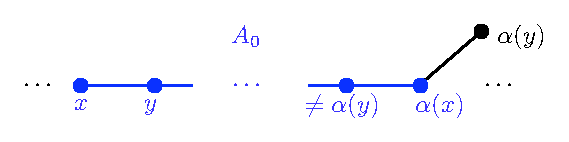
\includegraphics{grugraImages/A0}
\end{center}
Dann muss $\alpha(y)$ ein Nachbar von $\alpha(x)$ sein, aber
zugleich nicht in $A_0$ liegen, da sonst $d_0$ nicht minimal wäre.
Induktiv kann man so schließen:
\[
\alpha(A_0) \cap A_0 = \{\alpha(x)\}.
\]
Das ganze lässt sich nun für $\alpha(x)$ wiederholen, so dass wir
die Achse
\[
A(\alpha) := \BCUP{}{n\in\ZZ} \alpha^n(A_0)
\]
erhalten. Zur Eindeutigkeit kann man sich Folgendes überlegen:
Sei $z\not\in A(\alpha)$. Dann \glqq projiziere\grqq\ $z$ auf
$A(\alpha)$ durch den eindeutigen kürzesten Weg $\bar{zx_0}$
für ein geeignetes $x_0\in A(\alpha)$.
\begin{center}
	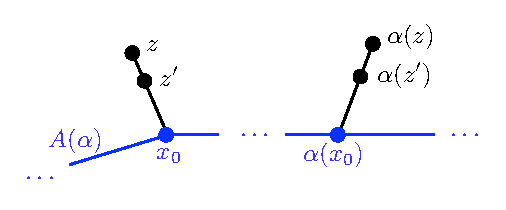
\includegraphics{grugraImages/Aalpha}
\end{center}
Betrachtet man einen Nachbarn $z'$ von $z$ in $\bar{zx_0}$, so
wird dieser Nachbar auf einen Nachbarn von $\alpha(z)$ zwischen
$\alpha(x_0)$ und $\alpha(z)$ abgebildet, kann also nicht
\glqq geschoben\grqq\ werden.
\qed

Fixpunkte eines Elementes $g\in\PGL_2(\QQ_p)$ sind Lösungen
von
\[
g(z)=\frac{az+b}{cz+d}=z \qquad \lra \qquad
cz^2+dz=az+b.
\]

Wir geben nun eine
\emph{Klassifikation der Elemente von $\boldsymbol{\PGL_2(\QQ_p)}$}
\index{Klassifikation in $\PGL_2(\QQ_p)$}
anhand ihrer Fixpunkte.

1. Fall: $c=0$. Ein Fixpunkt ist $\infty$.
\begin{itemize}
\item Falls $d\neq a$, so ist $\frac{b}{a-d}$ ein weiterer Fixpunkt.
\item Falls $d=a$ und $b=0$, so ist $g=\id$, also ist jeder
Punkt ein Fixpunkt.
\item Falls $d=a$ und $b\neq 0$, so ist $g$ eine Translation,
d.h. $\infty$ ist der einzige Fixpunkt.
\end{itemize}

2. Fall: $c\neq 0$. Die Lösungen der Fixpunktgleichung sind
durch
\[
\frac{a-d}{2c}\pm \frac{1}{2c}\sqrt{(a-d)^2+4bc}
\]
gegeben. Wir betrachten den Term unter der Wurzel:
\begin{align*}
(a-d)^2+4bc &= a^2+d^2-4ad+4bc+2ad \\
&= (a+d)^2 - 4 \det(g) \\
&=\spur(g)^2 - 4 \det(g).
\end{align*}
Die Spur und die Determinante von $g$ sind natürlich durch einen
Vertreter in $\GL_2(\QQ_p)$ gegeben.
Man überzeugt sich leicht, dass beim folgenden
Vergleich von $\spur(g)^2$ mit $4\det(g)$ die Wahl des
Vertreters unerheblich ist.
\begin{itemize}
\item $\spur(g)^2=4\det(g)$: In diesem Fall hat $g$
genau einen Fixpunkt in $\QQ_p$, nämlich $\frac{a-d}{2c}$.
\item $|\spur(g)^2|>|4\det(g)|$: In diesem Fall liegen
beide Fixpunkte von $g$ in $\QQ_p$ (nach dem Lemma von Hensel,
siehe van der Waerden \cite{vdW}, § 144).
\item $|\spur(g)^2|\leq|4\det(g)|$, aber
$\spur(g)^2\neq 4\det(g)$: In diesem Fall hat $g$
zwei Fixpunkte in der Erweiterung
$\QQ_p(\sqrt{\spur(g)^2-4\det(g)})$.
\end{itemize}

\BEM Die Eigenwerte von
$g=\begin{pmatrix}a&b\\ c&d\end{pmatrix}$
sind Lösungen der charakteristischen Gleichung
\[
\det
\begin{pmatrix}a-\lambda&b\\ c&d-\lambda\end{pmatrix}
=
\lambda^2 - \lambda(a+d) - bc + ad = 0.
\]
Die Eigenwerte sind also
\[
\frac{a+d}{2} \pm \sqrt{\spur(g)^2 - 4\det(g)},
\]
d.h. $g$ hat genau dann zwei verschiedene Fixpunkte,
wenn $g$ zwei verschiedene Eigenwerte hat.

\DB\ \begin{enumerate}
\item Hat $g$ nur einen Fixpunkt, so heißt $g$
\emph{parabolisch}\index{parabolisch} und ist konjugiert zu
$z\mapsto z+z_0$ für ein
$z_0\in\QQ_p^\times\backslash(\QQ_p^\times)^2$.
\item $g$ haben zwei verschieden Fixpunkte (also zwei
verschiedene Eigenwerte).
Haben die beiden Eigenwerte von $g$ den gleichen Betrag, so
heißt $g$ \emph{elliptisch}\index{elliptisch}, andernfalls
\emph{hyperbolisch}\index{hyberbolisch}.
\item Ist $|\spur(g)^2|>|4\det(g)|$, so ist $g$
hyperbolisch und konjugiert zu $z\mapsto\lambda z$ für ein
$\lambda\in\QQ_p$, $|\lambda|>1$ (denn falls $|\lambda|<1$,
konjugiere mit $\begin{pmatrix}0&1\\ -1&0\end{pmatrix}$).
\item Ist $|\spur(g)^2|\leq 4|\det(g)|$, so ist $g$
(parabolisch oder) elliptisch, und in\\
$\PGL_2(\QQ_p(\sqrt{\spur(g)^2-4\det(g)}))$ konjugiert
zu $z\mapsto \lambda z$ mit $|\lambda|=1$.
\end{enumerate}

\BEM\ \label{bem_hep}
\begin{enumerate}
\item Ist $g\in\PGL_2(\QQ_p)$ hyperbolisch, so gibt es eine
Achse $A_g$ in $T_p$, auf der $g$ durch Translation um
$\vv(\lambda)(=\lfloor\log_p|\lambda|\rfloor)\neq 0$ operiert.
\item Ist $g$ parabolisch, so hat $g$ genau ein Fixende
und viele Fixpunkte, aber keine Fixachse.
\item Ist $g$ elliptisch mit Fixpunkten in $\QQ_p$, so gibt es
eine Achse $A_g$ in $T_p$, die puntkweise fix ist unter
der Aktion von $g$.
\item Ist $g$ elliptisch mit Fixpunkten in $\QQ_p(\sqrt{p})$,
so invertiert $g$ eine Kante in $T_p$.
\item Ist $g$ elliptisch mit Fixpunkten in $\QQ_p(\sqrt{a})$,
$a\in\ZZ_p^\times\backslash(\ZZ_p^\times)^2$, $a\neq p$,
so fixiert $g$
genau eine Ecke in $T_p$, nämlich $\KU_{|z_1-z_2|}(z_1)$, wobei
$z_1, z_2$ die Fixpunkte sind.
\end{enumerate}

\SATZ\label{satz_ihara} \emph{(Satz von Ihara)}\index{Satz!Ihara}\index{Iharas Satz}\\
Ist $G\leq\PGL_2(\QQ_p)$ und jedes Element
$g\in G\backslash\{\id\}$ hyperbolisch,
so ist $G$ eine freie Gruppe.

\bew Nach Proposition \ref{prop_fp_achse} und
Bemerkung \ref{bem_hep}(1)
kann kein Element von $G\backslash\{\id\}$ einen Fixpunkt haben,
also operiert $G$ frei auf dem Baum $T_p$.
Nach Satz \ref{satz_frei} ist $G$ eine freie Gruppe.
\qed

\BSP Es seien $\KU_1$, $\KU_1'$ Ecken in $T_p$, so dass
$\KU_1\cap\KU_1'=\emptyset$ gilt.
Gesucht ist $g_1\in\PGL_2(\QQ_p)$ mit $g_1(\KU_1)=\KU_1'$ und
$\bar{\KU_1 \KU_1'}\subset A_{g_1}$.
Es seien $a,b,a',b'$ Enden in $T_p$ mit
$\KU_1=\med(a,b,\infty)$ und $\KU_1'=\med(a',b',\infty)$
(vgl. Abbildung weiter unten).
Wähle $g_1$ so, dass
\begin{align*}
g_1(a) &= a,\\
g_1(b) &= b',\\
g_1(a') &= a'
\end{align*}
gilt. Dann gilt $g(\KU_1)=\KU_1'$, denn für ein weiteres $c\in\KU_1$
ist $g(c)\in\KU_1'$, da $g(A_{a,\infty})=A_{a',\infty}$.
(Beachte, dass $g_1$ zwar
Fixpunkte in $\PP^1(\QQ_p)$ hat, aber nicht auf $T_p$.)
\begin{center}
	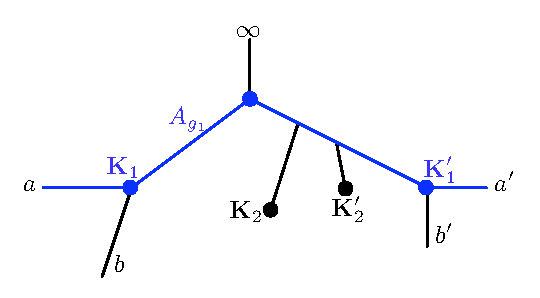
\includegraphics{grugraImages/ihara1}
\end{center}
Nun seien $\KU_2$ und $\KU_2'$ weitere Kreise, so dass
$\KU_1,\KU_1',\KU_2,\KU_2'$ paarweise disjunkt sind.
Es sei $g_2\in\PGL_2(\QQ_p)$ mit $g_2(\KU_2)=\KU_2'$ und
$\bar{\KU_2 \KU_2'}\subset A_{g_2}$.

\textsl{Behauptung}: $G=\lag g_1, g_2 \rag$ ist eine freie Gruppe.

Wir werden unten zwei verschiedene Beweise dafür angeben.
Zunächst betrachten wir die Aktion von $g_1$ (und analog $g_2$)
genauer. Als Teilmenge von $\PP^1(\QQ_p)$ ist
\[
g_1(\KU_1) = \PP^1(\QQ_p) \backslash \KU_{|a'-b'|/p}(a').
\]
Also bildet $g_1$ den Rand von $\KU_1$  (bzgl. Mittelpunkt $a$) auf
den Rand von $\KU_1'$ (bzgl. Mittelpunkt $a'$) ab, und das Innere
von $\KU_1$ wird auf das Äußere von $\KU_1'$ abgebildet.

\textsc{Erster Beweis:}
(Dieser Beweis funktioniert analog zu einem entsprechenden
Resultat für $\PP^1(\CC)$.)
Es sei
$z\in\PP^1(\QQ_p)\backslash(\KU_1\cup\KU_1'\cup\KU_2\cup\KU_2')$,
und
\[
g = g_1^{\eps_1} g_2^{\delta_1} \cdots g_1^{\eps_n} g_2^{\delta_n}
\]
beliebiges reduziertes Wort in $g_1$ und $g_2$.
Dann gilt
\[
g(z) \in
\left\{
\begin{matrix}
\KU_1, & \eps_1<0 \\
\KU_1', &\eps_1>0 \\
\KU_2, &\eps_1=0,\delta_1<0\\
\KU_2', &\eps_1=0,\delta_1>0
\end{matrix}
\right..
\]
Also ist $g(z)\neq z$ und $g\neq\id$. Somit ist $G$ frei.
\qed

\textsc{Zweiter Beweis:} Es sei $F\subset T_p$ der von den Ecken
$\KU_1,\KU_1',\KU_2,\KU_2'$ aufgespannte Teilbaum, und
$\KU$ eine Ecke in $F\backslash\{\KU_1,\KU_1',\KU_2,\KU_2'\}$.
\begin{center}
	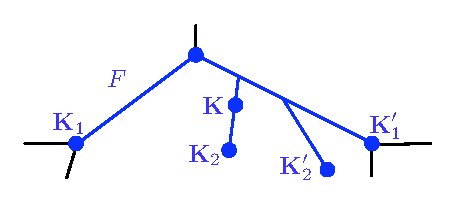
\includegraphics{grugraImages/ihara2}
\end{center}
Es sei
\[
g = g_1^{\eps_1} g_2^{\delta_1} \cdots g_1^{\eps_n} g_2^{\delta_n}
\]
ein beliebiges reduziertes Wort in $g_1$ und $g_2$.
Mit Induktion folgt $g(\KU)\not\in F$, also insbesondere
$g(\KU)\neq\KU$ und $g\neq \id$.
\qed

\BEM Es sei
\[
T_p(G):=\BCUP{}{g\in G} g F.
\]
$T_p(G)$ ist ein Baum und nach Konstruktion $G$-invariant.
$T_p(G)/G$ ist ein endlicher Graph und isomorph zu $F/\sim$, wobei
$\sim$ durch Identifizierung zweier Eckpunkte, die zu $g_i$ gehören,
gegeben ist.

\BEM Für jedes $\nu\geq 1$ gibt es in $\PGL_2(\QQ_p)$ (und in
$\PSL_2(\CC)$) eine Untergruppe $G$ mit:
\begin{itemize}
\item $G$ ist frei vom Rang $\nu$.
\item $G\backslash\{\id\}$ enthält nur hyperbolische Elemente.
\item Es gibt eine offene Teilmenge $F$ von $\PP^1(\QQ_p)$ (bzw.
$\PP^1(\CC)$) mit $g(F)\cap F=\emptyset$ für alle $g\in G$,
$g\neq\id$. Es ist
\[
F=\PP^1(\QQ_p)\backslash\BCUP{\nu}{i=1}(\KU_i\cup\KU_i').
\]
\end{itemize}
Eine solche Gruppe $G$ heißt \emph{Schottky-Gruppe}.\index{Gruppe!Schottky-}\index{Schottky-Gruppe}